% Created 2015-01-03 Sat 21:58
\documentclass[11pt]{article}
\usepackage[utf8]{inputenc}
\usepackage[T1]{fontenc}
\usepackage{fixltx2e}
\usepackage{graphicx}
\usepackage{longtable}
\usepackage{float}
\usepackage{wrapfig}
\usepackage{rotating}
\usepackage[normalem]{ulem}
\usepackage{amsmath}
\usepackage{textcomp}
\usepackage{marvosym}
\usepackage{wasysym}
\usepackage{amssymb}
\usepackage{hyperref}
\tolerance=1000
\usepackage[utf8]{inputenc}
\usepackage[usenames,dvipsnames]{color}
\usepackage[backend=bibtex, style=numeric]{biblatex}
\usepackage{commath}
\usepackage{tikz}
\usetikzlibrary{shapes,backgrounds}
\usepackage{marginnote}
\usepackage{listings}
\usepackage{color}
\usepackage{enumerate}
\hypersetup{urlcolor=blue}
\hypersetup{colorlinks,urlcolor=blue}
\addbibresource{bibliography.bib}
\setlength{\parskip}{16pt plus 2pt minus 2pt}
\definecolor{codebg}{rgb}{0.96,0.99,0.8}
\definecolor{codestr}{rgb}{0.46,0.09,0.2}
\author{Oleg Sivokon}
\date{\textit{<2015-01-02 Fri>}}
\title{Assignment 15, Introduction To Mathematics}
\hypersetup{
  pdfkeywords={Introduction To Mathematics, Assignment, Set Theory},
  pdfsubject={Fifth asssignment in the course Introduction To Mathematics},
  pdfcreator={Emacs 25.0.50.1 (Org mode 8.2.2)}}
\begin{document}

\maketitle
\tableofcontents


\lstset{ %
  backgroundcolor=\color{codebg},
  basicstyle=\ttfamily\scriptsize,
  breakatwhitespace=false,         % sets if automatic breaks should only happen at whitespace
  breaklines=false,
  captionpos=b,                    % sets the caption-position to bottom
  commentstyle=\color{mygreen},    % comment style
  framexleftmargin=10pt,
  xleftmargin=10pt,
  framerule=0pt,
  frame=tb,                        % adds a frame around the code
  keepspaces=true,                 % keeps spaces in text, useful for keeping indentation of code (possibly needs columns=flexible)
  keywordstyle=\color{blue},       % keyword style
  showspaces=false,                % show spaces everywhere adding particular underscores; it overrides 'showstringspaces'
  showstringspaces=false,          % underline spaces within strings only
  showtabs=false,                  % show tabs within strings adding particular underscores
  stringstyle=\color{codestr},     % string literal style
  tabsize=2,                       % sets default tabsize to 2 spaces
}

\clearpage

\section{Problems}
\label{sec-1}

\subsection{Problem 1}
\label{sec-1-1}

\begin{enumerate}
\item Let $A$ be a set and $f, g$ be functions defined over $A$.
Prove that if $f$ isn't surjective, so is the $f \circ g$.
\item Let $f$ and $g$ be functions from $\mathbb{N}$ to $\mathbb{N}$,
defined as follows:
\begin{equation*}
  f(n)= \begin{cases}
    \frac{n+1}{2} & \text{if $n$ is odd} \\
    1             & \text{otherwise}
  \end{cases}
  , \kern 30pt
  g(n)= 2n-1\
\end{equation*}

Prove that $g$ is not surjective, and yet $f \circ g$ is.

\item Let $A$ be a set and $f, g$ be functions defined on it.  Prove that if
$g$ is not surjective and $f$ is bijective, then $f \circ g$ is not
surjective either.
\end{enumerate}

\subsubsection{Answer 1}
\label{sec-1-1-1}
I will proceed proving this following this intuition: if the element is
not in the domain of $f$ then no matter what you compose $f$ with on the
left side, that element will not be in the domain of $f$ anyway.

Let's formalize this.  For a function to \emph{not} be surjective means that
there exists an element (let's call it $x$) in the domain of function
which has no match in the function's co-domain.  Now, suppse $g$ could
produce any element in the co-domain of $f$, there would still be no 
element in the domain of $f$ for $x$.
\subsubsection{Answer 2}
\label{sec-1-1-2}
Some observation first: It is easy to see that $g$ is the function that
generates all odd numbers.  All even numbers in the domain of $f$ as well as
odds have an element in its co-domain.  So, if we prove the equivalent
statement: all odd numbers in the co-domain of $f \circ g$ have a match in
the domain of $f \circ g$ we had proved the original statement as well.

But before we proceed, let's establish that $g$ is not surjective
(as required by the problem statement).  Clearly no even number in the
co-domain of $g$ has a match in its domain.  This contradicts the
definition of surjection.

Now, let's substitute $g$ into the definition of $f$ to obtain $f \circ g$:

\begin{equation*}
  (f \circ g)(n)= \begin{cases}
    \frac{2n-1+1}{2} & \text{if $n$ is odd} \\
    1                & \text{otherwise}
  \end{cases}=\begin{cases}
    n & \text{if $n$ is odd} \\
    1 & \text{otherwise}
  \end{cases}
\end{equation*}

Clearly, this function matches every even element with 1.  That being
proved we proved the problem statement as well.
\subsubsection{Answer 3}
\label{sec-1-1-3}
The intuition for the proof is that if elements of the domain of $g$ are
missing some particular element, then, if $f$ is a bijection it would
have to be missing the element which it matches to the missing one (and
it has to assign a \emph{unique} element to it, because it is a bijection).

I will proceed by contradiction.  I will assume that for some element $x$
in the domain of $g$ there is no match in the co-domain of $g$.  Now
since $f$ is a bijectin, it follows that it matches $x$ with $x'$ in its
domain.  Since $f$ is a function, it can only match one element to $x$,
i.e. there is at most one $x'$, and it necessary that $x'$ exists,
otherwise $f$ wouldn't be a bijection.  So, it is necessary that if $x'$
is in $A$, so should be $x$ (by definition of $f$) in the domain of $g$,
but we started this proof by assuming that $x$ is not in the domain of
$g$.  Having arrived at contradiction I conclude that the initial
assumption must be true.
\subsection{Problem 2}
\label{sec-1-2}
Let $ABCD$ be a rectangle with its center in $O$ (as seen in the image below).

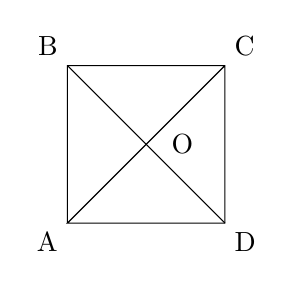
\begin{tikzpicture}
  \draw
  (0,0) coordinate (A) node[below left] {A}
  -- (0,2) coordinate (B) node[above left] {B}
  -- (2,2) coordinate (C) node[above right] {C}
  -- (2,0) coordinate (D) node[below right] {D}
  -- (A) -- (C);
  \draw (B) -- (D);
  \draw (1.2,1) coordinate node[right] {O};
\end{tikzpicture}

And let $f$ be an isometry such that $\{A,B,C,D\}$ is its fixed set, while
$ABCD$ is a square with its center in $O$.  $f$ is an isometry defined
on $\{A,B,C,D\}$ such that $f(C)=A$.

\begin{enumerate}
\item Prove that $f(A)=C$ and that $O$ is the fixed point of $f$.
\item Prove that if $f(B)=B$, then $f$ is a reflection.
\item Prove that if $f(B)=C$, then $f$ is a rotation.
\item Prove that $f$ cannot send $B$ neither to $A$ nor to $C$.
\end{enumerate}

\subsubsection{Answer 3}
\label{sec-1-2-1}
As the first step, I shall narrow down possible candidates for this isometry:
We can immediately discard a possibility that $f$ is a translation - because,
were it a translatin, $f(B)$ would not be positioned on either of the vertices
of $ABCD$, and then by pigeonhole principle, we would not be able to produce
enough fixed points using this transformation.  In other words, if $f$ was a
translation, it would have $l$ equal to the diagonal of $ABCD$ and $\alpha$
equal $\frac{\pi}{2}$ relative to the diagonal $BD$.  Applying the same
transformation to $B$ clearly won't put it neither into $A$ not into $D$.

By the similar reasoning $f$ can't be a reflection with translation.  I.e. if
we chose to move $A$ to $C$ accross any line that isn't parallel with diagonal
$BD$, we would end up with $B$ not lending on any of the fixed points of the
$ABCD$ after we applied $f$ to it.

Trivially, this can't be an identity transformation, since it doesn't send
$A$ to $A$.

Thus, we are left with two possibilities:
\begin{enumerate}
\item $f$ is a rotation.
\item $f$ is a reflection.
\end{enumerate}

We can now simply examine all possible cases of translation of the remaining
points.  Since $f$ is a bijection and a surjection, we know that there is
only one point it can send any point to.  We also just proved that it can't
send A to itself (if it did the $\overline{AC} \neq \overline{f(A)f(C)}$.
Hence, the possibilities are:
\begin{enumerate}
\item $A$ is sent to $C$.
\item $A$ is sent to $B$.
\item $A$ is sent to $D$.
\end{enumerate}

It is easy to see that in order to preserve the distance $\overline{AC}$ we
must choose to send $A$ to $C$.  Otherwise $f(A)$ ends up connected to $C$
by the side of the square, which is not equal to the original diagonal of
the same square.

Now, let's prove that $O$ is indeed the fixed point of $f$.  Since we already
konw that $f(A)=C$, we are only left with two possible translations of $B$
and $D$:
\begin{enumerate}
\item $f(B)=B$, $f(D)=D$.
\item $f(B)=D$, $f(D)=B$.
\end{enumerate}

In case 1, this is a reflection along the diagonal $BD$.  This is so because
only reflection (of all the options that we are left with) can have more than
one fixed point (observe that $B$ and $D$ under $f$, if it is a reflection are
fixed).  Since $O$ lies on the diagonal $BD$ by construction, it is, by
definition of reflection is its fixed point.

In case 2, this is a rotation by $\pi$ around $O$.  The readers may convince
themselves of this in the following way:  By construction, $OA=OB=OC=OD$,
$\angle AOC = \angle DOB = \angle COB = \angle BOD$.  These are the ohly
possible angles, given $O$ is a center of isometry $f$, provided $f$ is
a rotation, with the radius being haf the diagonal of $ABCD$.

Thus, $O$ is the fixed point of $f$ and $f(A)=C$.
\subsubsection{Answer 4}
\label{sec-1-2-2}
I had proved this eventually during \ref{sec-1-2-1}.  Just to restate the proof
briefly:  $f(B)=B \implies f(D)=D$, but only reflection (of the remaining
possible options) can afford multiple fixed points.
\subsubsection{Answer 5}
\label{sec-1-2-3}
Again, I have showed this already during \ref{sec-1-2-1}, but to make this more
comprehensive: I listed all possible angles and radii that would have been
produced by such isometry, and, comparing them to each other become
convinced that they satisfy the requirement for rotation.
\subsubsection{Answer 6}
\label{sec-1-2-4}
Sending $B$ to either $A$ or $C$ would require the distance $\overline{AB}$
or $\overline{BC}$ to be preserved under this transformation (otherwise it
would not be an isometry).  But this is not possible because
$\overline{f(A)f(B)}=\overline{AA}=0$, but $\overline{AB} \neq 0$. The proof
for $\overline{BC}$ is identical.
\subsection{Problem 3}
\label{sec-1-3}
Let $f$ and $g$ be isometries on a surface, s.t. $f'=g \circ f \circ g^{-1}$.

\begin{enumerate}
\item Prove that $f'$ is an isometry and that $f'$ preserves direction iff
so does $f$.
\item Prove that if $A$ is a fixed point of isometry $f$, then $g(A)$ must
be a fixed point of isometry $f'$.  And if $B$ is a fixed point of
$f'$, then $g^{-1}(B)$ is a fixed point of $f$.
\item Prove that $f$ and $f'$ are of the same kind.
\end{enumerate}

\subsubsection{Answer 7}
\label{sec-1-3-1}
\subsubsection{Answer 8}
\label{sec-1-3-2}
\subsubsection{Answer 9}
\label{sec-1-3-3}
\subsection{Problem 4}
\label{sec-1-4}
Shown in the picture below are three lines: $\ell_1, \ell_2, \ell_3$
all parallel and $\ell_4$ which intersects with them.

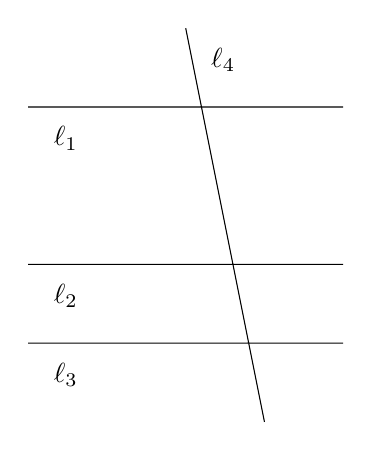
\begin{tikzpicture}
  \draw
  (0,1) -- (4,1)
  (0,2) -- (4,2)
  (0,4) -- (4,4)
  (3,0) -- (2,5);
  \draw (0.2,0.6) node[right] {$\ell_3$};
  \draw (0.2,1.6) node[right] {$\ell_2$};
  \draw (0.2,3.6) node[right] {$\ell_1$};
  \draw (2.2,4.6) node[right] {$\ell_4$};
\end{tikzpicture}

\begin{enumerate}
\item Prove that $S_{\ell_4} \circ S_{\ell_3} \circ S_{\ell_2} \circ S_{\ell_1}$
is a rotation.
\item Prove that $S_{\ell_4} \circ S_{\ell_3} \circ S_{\ell_2} \circ S_{\ell_1}=
      S_{\ell_4} \circ S_{\ell_1} \circ S_{\ell_2} \circ S_{\ell_3}$.
\end{enumerate}
% Emacs 25.0.50.1 (Org mode 8.2.2)
\end{document}